\documentclass[]{article}
\usepackage[T1]{fontenc}
\usepackage{lmodern}
\usepackage{amssymb,amsmath}
\usepackage{ifxetex,ifluatex}
\usepackage{fixltx2e} % provides \textsubscript
% use upquote if available, for straight quotes in verbatim environments
\IfFileExists{upquote.sty}{\usepackage{upquote}}{}
\ifnum 0\ifxetex 1\fi\ifluatex 1\fi=0 % if pdftex
  \usepackage[utf8]{inputenc}
\else % if luatex or xelatex
  \ifxetex
    \usepackage{mathspec}
    \usepackage{xltxtra,xunicode}
  \else
    \usepackage{fontspec}
  \fi
  \defaultfontfeatures{Mapping=tex-text,Scale=MatchLowercase}
  \newcommand{\euro}{€}
\fi
% use microtype if available
\IfFileExists{microtype.sty}{\usepackage{microtype}}{}
\usepackage[margin=1in]{geometry}
\usepackage{color}
\usepackage{fancyvrb}
\newcommand{\VerbBar}{|}
\newcommand{\VERB}{\Verb[commandchars=\\\{\}]}
\DefineVerbatimEnvironment{Highlighting}{Verbatim}{commandchars=\\\{\}}
% Add ',fontsize=\small' for more characters per line
\usepackage{framed}
\definecolor{shadecolor}{RGB}{248,248,248}
\newenvironment{Shaded}{\begin{snugshade}}{\end{snugshade}}
\newcommand{\KeywordTok}[1]{\textcolor[rgb]{0.13,0.29,0.53}{\textbf{{#1}}}}
\newcommand{\DataTypeTok}[1]{\textcolor[rgb]{0.13,0.29,0.53}{{#1}}}
\newcommand{\DecValTok}[1]{\textcolor[rgb]{0.00,0.00,0.81}{{#1}}}
\newcommand{\BaseNTok}[1]{\textcolor[rgb]{0.00,0.00,0.81}{{#1}}}
\newcommand{\FloatTok}[1]{\textcolor[rgb]{0.00,0.00,0.81}{{#1}}}
\newcommand{\CharTok}[1]{\textcolor[rgb]{0.31,0.60,0.02}{{#1}}}
\newcommand{\StringTok}[1]{\textcolor[rgb]{0.31,0.60,0.02}{{#1}}}
\newcommand{\CommentTok}[1]{\textcolor[rgb]{0.56,0.35,0.01}{\textit{{#1}}}}
\newcommand{\OtherTok}[1]{\textcolor[rgb]{0.56,0.35,0.01}{{#1}}}
\newcommand{\AlertTok}[1]{\textcolor[rgb]{0.94,0.16,0.16}{{#1}}}
\newcommand{\FunctionTok}[1]{\textcolor[rgb]{0.00,0.00,0.00}{{#1}}}
\newcommand{\RegionMarkerTok}[1]{{#1}}
\newcommand{\ErrorTok}[1]{\textbf{{#1}}}
\newcommand{\NormalTok}[1]{{#1}}
\usepackage{graphicx}
% Redefine \includegraphics so that, unless explicit options are
% given, the image width will not exceed the width of the page.
% Images get their normal width if they fit onto the page, but
% are scaled down if they would overflow the margins.
\makeatletter
\def\ScaleIfNeeded{%
  \ifdim\Gin@nat@width>\linewidth
    \linewidth
  \else
    \Gin@nat@width
  \fi
}
\makeatother
\let\Oldincludegraphics\includegraphics
{%
 \catcode`\@=11\relax%
 \gdef\includegraphics{\@ifnextchar[{\Oldincludegraphics}{\Oldincludegraphics[width=\ScaleIfNeeded]}}%
}%
\ifxetex
  \usepackage[setpagesize=false, % page size defined by xetex
              unicode=false, % unicode breaks when used with xetex
              xetex]{hyperref}
\else
  \usepackage[unicode=true]{hyperref}
\fi
\hypersetup{breaklinks=true,
            bookmarks=true,
            pdfauthor={Gildardo Rojas Nandayapa},
            pdftitle={Regression Models - Course Project},
            colorlinks=true,
            citecolor=blue,
            urlcolor=blue,
            linkcolor=magenta,
            pdfborder={0 0 0}}
\urlstyle{same}  % don't use monospace font for urls
\setlength{\parindent}{0pt}
\setlength{\parskip}{6pt plus 2pt minus 1pt}
\setlength{\emergencystretch}{3em}  % prevent overfull lines
\setcounter{secnumdepth}{0}

\title{Regression Models - Course Project}
\author{Gildardo Rojas Nandayapa}
\date{Saturday, October 25, 2014}

\begin{document}

\begin{center}
\huge Regression Models - Course Project \\[0.2cm]
\end{center}
\begin{center}
\large \emph{Gildardo Rojas Nandayapa}\\[0.1cm]
\end{center}
\begin{center}
\large \emph{Saturday, October 25, 2014} \\
\end{center}
\normalsize


\subsection{Executive Summary}\label{executive-summary}

Motor Trend, a leading magazine about the automobile industry is
interested in looking at a data set of a collection of cars, exploring
the relationship between a set of variables and miles per gallon (MPG).
There is particular interest in the following two questions:

\begin{enumerate}
\def\labelenumi{\arabic{enumi}.}
\itemsep1pt\parskip0pt\parsep0pt
\item
  Is an automatic or manual transmission better for MPG?
\item
  What is the difference in MPG between automatic and manual
  transmissions?
\end{enumerate}

Using linear regression analysis, we can determine that there is a
signficant difference between the mean MPG for automatic and manual
transmission cars. Manual transmissions achieve a higher value of MPG
compared to automatic transmission.

Transmission type is relevant, but not an unique factor predicting the
mpg outcome as we may see in the following analysis.

\subsection{The Data}\label{the-data}

The data was extracted from the 1974 Motor Trend US magazine, it
comprises fuel consumption and 10 aspects of automobile design and
performance for 32 automobiles (1973-74 models).

\subsection{Exploratory Analysis}\label{exploratory-analysis}

This study is focused on the effects of car transmission type over mpg
efficiency, so a simple box plot may help to depict the difference
between cars with automatic and manual transmission. The plot shows that
manual transmissions have higher mpg. See \textbf{Appendix - Figure 1.
MPG by Transmission Type - Box plot}

To find relationships between all variables, data exploration can be
extended visually using the pairs plot. By inspecting the plot we may
notice variables related to mpg, though the impact varies in magnitude
and slope. See \textbf{Appendix - Figure 2. Motor Trend Car Road Tests -
Variable pairs plot.}

\subsubsection{Statistical Inference}\label{statistical-inference}

\textbf{T-test} Assuming a normal distribution, by performing a t-test
we may observe that there is a significant difference between manual and
automatic transmission types in the resulting mpg.

\begin{Shaded}
\begin{Highlighting}[]
\KeywordTok{data}\NormalTok{(mtcars)}
\KeywordTok{t.test}\NormalTok{(mpg ~}\StringTok{ }\NormalTok{am, }\DataTypeTok{data =} \NormalTok{mtcars)}
\end{Highlighting}
\end{Shaded}

\begin{verbatim}
## 
##  Welch Two Sample t-test
## 
## data:  mpg by am
## t = -3.767, df = 18.33, p-value = 0.001374
## alternative hypothesis: true difference in means is not equal to 0
## 95 percent confidence interval:
##  -11.28  -3.21
## sample estimates:
## mean in group 0 mean in group 1 
##           17.15           24.39
\end{verbatim}

Here we may also observe that the difference in mpg for vehicles with
manual over automatic transmission type is 7.24.

\subsection{Regression Analysis}\label{regression-analysis}

\subsubsection{Linear Regression}\label{linear-regression}

First we attempt simple linear regression.

\begin{Shaded}
\begin{Highlighting}[]
\NormalTok{fit <-}\StringTok{ }\KeywordTok{lm}\NormalTok{(mpg ~}\StringTok{ }\NormalTok{am, }\DataTypeTok{data=}\NormalTok{mtcars)}
\KeywordTok{summary}\NormalTok{(fit)}
\end{Highlighting}
\end{Shaded}

\begin{verbatim}
## 
## Call:
## lm(formula = mpg ~ am, data = mtcars)
## 
## Residuals:
##    Min     1Q Median     3Q    Max 
## -9.392 -3.092 -0.297  3.244  9.508 
## 
## Coefficients:
##             Estimate Std. Error t value Pr(>|t|)    
## (Intercept)    17.15       1.12   15.25  1.1e-15 ***
## am              7.24       1.76    4.11  0.00029 ***
## ---
## Signif. codes:  0 '***' 0.001 '**' 0.01 '*' 0.05 '.' 0.1 ' ' 1
## 
## Residual standard error: 4.9 on 30 degrees of freedom
## Multiple R-squared:  0.36,   Adjusted R-squared:  0.338 
## F-statistic: 16.9 on 1 and 30 DF,  p-value: 0.000285
\end{verbatim}

Observing the summary information, we can confirm that manual
transmission vehicles have 7.24 MPG more than automatic ones. But this
model doesn't provide complete information as the Multiple R-squared
value of .3598 means the model can just explain 35.98\% of the variance.

In order to fully understand the transmission type impact considering
other variables, we need to create a multivariate model.

\subsubsection{Building and selecting the
Model}\label{building-and-selecting-the-model}

To start, we build the first model which considers all variables as
predictors. Then we proceed to select the most significant predictors to
build the best model.

The step function performs the best model selection, it calls lm
repeatedly to build regression models selecting the most significant
variables that can be considered as relevant mpg predictors, while
discarding the less significant ones.

\begin{Shaded}
\begin{Highlighting}[]
\NormalTok{firstmodel <-}\StringTok{ }\KeywordTok{lm}\NormalTok{(mpg ~}\StringTok{ }\NormalTok{., }\DataTypeTok{data=}\NormalTok{mtcars)}
\NormalTok{bestmodel <-}\StringTok{ }\KeywordTok{step}\NormalTok{(firstmodel, }\DataTypeTok{direction=}\StringTok{"both"}\NormalTok{, }\DataTypeTok{trace=}\DecValTok{0}\NormalTok{)}
\KeywordTok{summary}\NormalTok{(bestmodel)}
\end{Highlighting}
\end{Shaded}

\begin{verbatim}
## 
## Call:
## lm(formula = mpg ~ wt + qsec + am, data = mtcars)
## 
## Residuals:
##    Min     1Q Median     3Q    Max 
## -3.481 -1.556 -0.726  1.411  4.661 
## 
## Coefficients:
##             Estimate Std. Error t value Pr(>|t|)    
## (Intercept)    9.618      6.960    1.38  0.17792    
## wt            -3.917      0.711   -5.51    7e-06 ***
## qsec           1.226      0.289    4.25  0.00022 ***
## am             2.936      1.411    2.08  0.04672 *  
## ---
## Signif. codes:  0 '***' 0.001 '**' 0.01 '*' 0.05 '.' 0.1 ' ' 1
## 
## Residual standard error: 2.46 on 28 degrees of freedom
## Multiple R-squared:  0.85,   Adjusted R-squared:  0.834 
## F-statistic: 52.7 on 3 and 28 DF,  p-value: 1.21e-11
\end{verbatim}

\begin{Shaded}
\begin{Highlighting}[]
\KeywordTok{anova}\NormalTok{(firstmodel,bestmodel)}
\end{Highlighting}
\end{Shaded}

\begin{verbatim}
## Analysis of Variance Table
## 
## Model 1: mpg ~ cyl + disp + hp + drat + wt + qsec + vs + am + gear + carb
## Model 2: mpg ~ wt + qsec + am
##   Res.Df RSS Df Sum of Sq    F Pr(>F)
## 1     21 148                         
## 2     28 169 -7     -21.8 0.44   0.86
\end{verbatim}

By displaying the model summary, we can see that Weight and Accelaration
are also relevant to predict mpg. Here the Multiple R-squared value of
.8497 means the model can now explain 84.97\% of the mpg variance,
making it a better predictive model. We also computed the analysis of
variance (or deviance) tables for one the previously fitted models
(firstmodel and bestmodel).

\subsubsection{Analysis of residuals}\label{analysis-of-residuals}

Now with the model selection done, we proceed with the analysis of
residuals. While reading the following observations, please see
\textbf{Figure 3 - Residual plots.}

\textbf{Observations}

\textbf{Residual vs Fitted plot} The independence condition may be
confirmed with the randomly scatterd points that this plot shows.

\textbf{Normal Q-Q plot} Normal distribution of residuals can be
confirmed as most points fall in the line.

\textbf{Scale-Location plot} Constant variance can be observed as points
are scattered in a constant band.

\textbf{Residuals vs Leverage plot} In this plot we can observe some
outliers or leverage points, the points in the top right may indicate
values with increased leverage of outliers. We will also perform of
regression diagnostics using the function hatvalues() to find data
points with most leverage and dfbetas() to find the data points that
have bigger influence in the model coefficients.

\begin{Shaded}
\begin{Highlighting}[]
\NormalTok{leverage <-}\StringTok{ }\KeywordTok{hatvalues}\NormalTok{(bestmodel)}
\KeywordTok{tail}\NormalTok{(}\KeywordTok{sort}\NormalTok{(leverage),}\DecValTok{3}\NormalTok{)}
\end{Highlighting}
\end{Shaded}

\begin{verbatim}
##   Chrysler Imperial Lincoln Continental            Merc 230 
##              0.2296              0.2642              0.2970
\end{verbatim}

\begin{Shaded}
\begin{Highlighting}[]
\NormalTok{influential <-}\StringTok{ }\KeywordTok{dfbetas}\NormalTok{(bestmodel)}
\KeywordTok{tail}\NormalTok{(}\KeywordTok{sort}\NormalTok{(influential[,}\DecValTok{4}\NormalTok{]),}\DecValTok{3}\NormalTok{)}
\end{Highlighting}
\end{Shaded}

\begin{verbatim}
##     Toyota Corona          Fiat 128 Chrysler Imperial 
##            0.4050            0.4766            0.5626
\end{verbatim}

\subsection{Conclusions}\label{conclusions}

\begin{itemize}
\itemsep1pt\parskip0pt\parsep0pt
\item
  MT Vehicles are better to get more MPG compared with AT vehicles.
\item
  MT vehicles have in average 7.24 MPG more than AT vehicles.
\item
  Transmission Type has relevance as a predictor for MPG result, but
  there are other variables like Weight and Acceleration (wt and qseq)
  that also have strong influence predicting the mpg outcome.
\item
  The model generated in this analysis has an 85\% of accuracy adjusted
  to the above mentioned variables.
\end{itemize}

\subsubsection{Apendix}\label{apendix}

\begin{Shaded}
\begin{Highlighting}[]
\KeywordTok{boxplot}\NormalTok{(mpg ~}\StringTok{ }\NormalTok{am, }\DataTypeTok{data=}\NormalTok{mtcars, }\DataTypeTok{ylab=}\StringTok{"Miles per Gallon"}\NormalTok{, }\DataTypeTok{xlab=}\StringTok{"Transmission Type (0=AT, 1=MT)"}\NormalTok{, }\DataTypeTok{col=}\NormalTok{(}\KeywordTok{c}\NormalTok{(}\StringTok{"blue"}\NormalTok{,}\StringTok{"green"}\NormalTok{)))}
\end{Highlighting}
\end{Shaded}

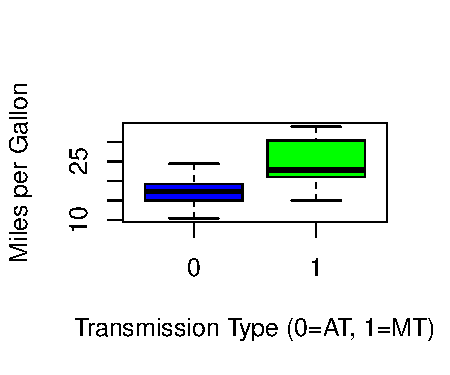
\includegraphics{./Regression_Models_-_Course_Project_5_pages_files/figure-latex/smallplot.pdf}

\textbf{Figure 1. MPG by Transmission Type - Box plot}

\begin{Shaded}
\begin{Highlighting}[]
\KeywordTok{require}\NormalTok{(stats); }\KeywordTok{require}\NormalTok{(graphics)}
\KeywordTok{pairs}\NormalTok{(mtcars, }\DataTypeTok{pane=}\NormalTok{panel.smooth, }\DataTypeTok{main=}\StringTok{"Motor Trend Car Road Tests"}\NormalTok{, }\DataTypeTok{col=}\DecValTok{3}\NormalTok{)}
\end{Highlighting}
\end{Shaded}

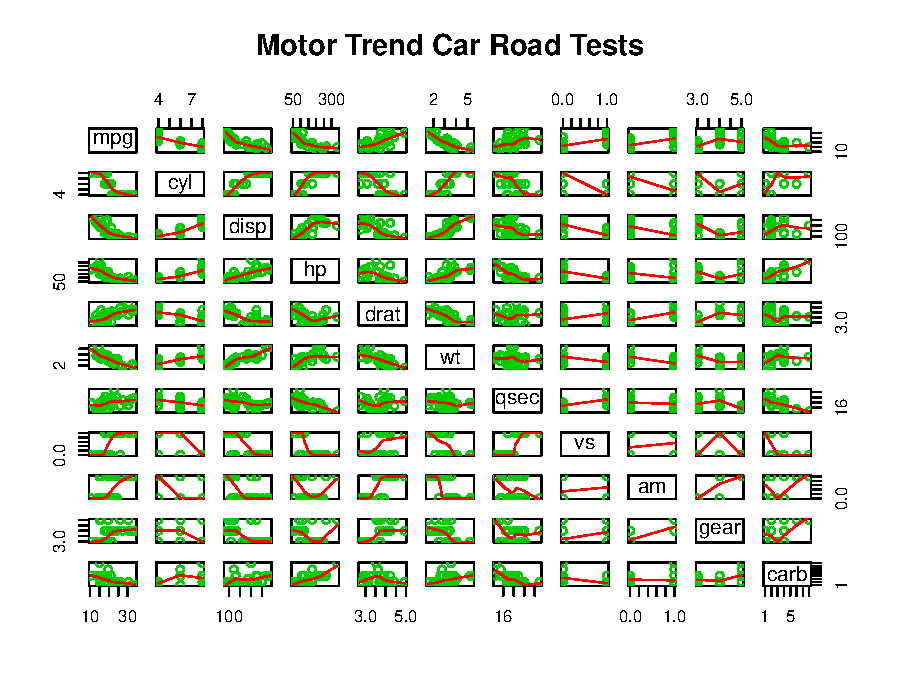
\includegraphics{./Regression_Models_-_Course_Project_5_pages_files/figure-latex/unnamed-chunk-5.pdf}

\textbf{Figure 2. Motor Trend Car Road Tests - Variable pairs plot}

\begin{Shaded}
\begin{Highlighting}[]
\KeywordTok{par}\NormalTok{(}\DataTypeTok{mfrow=}\KeywordTok{c}\NormalTok{(}\DecValTok{2}\NormalTok{, }\DecValTok{2}\NormalTok{))}
\KeywordTok{plot}\NormalTok{(bestmodel)}
\end{Highlighting}
\end{Shaded}

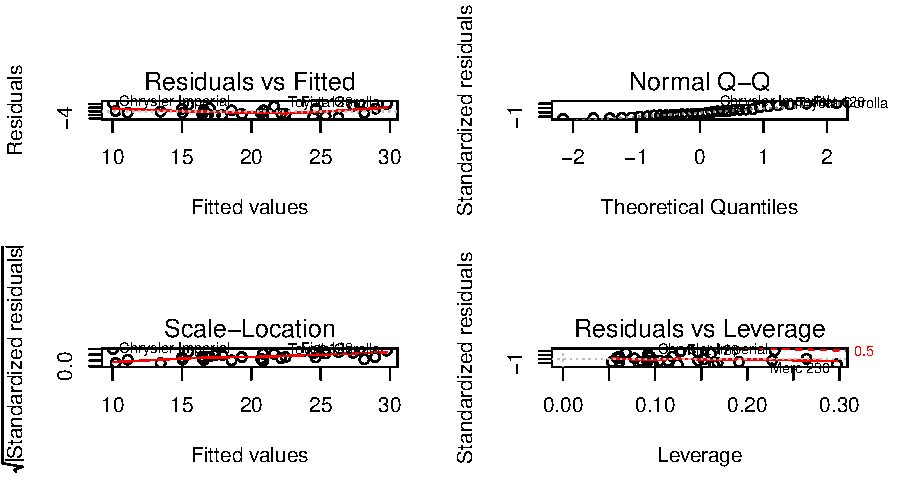
\includegraphics{./Regression_Models_-_Course_Project_5_pages_files/figure-latex/unnamed-chunk-6.pdf}

\textbf{Figure 3. Residual Plots}

\end{document}
